\documentclass{article}
\usepackage[a4paper, margin=3mm, landscape]{geometry}
\usepackage{multicol}
\usepackage{xcolor}
\usepackage{enumitem}
\usepackage{amsmath}
\usepackage{amsfonts}
\usepackage{listings}
\usepackage{soul}
\usepackage{graphicx}

\pdfinfo{
    /Title (ACC1701x.pdf)
    /Creator (TeX)
    /Producer (pdfTeX 1.40.0)
    /Author (Vincent Pang)
    /Subject (CS2106)
    /Keywords (CS2106, nus, cheatsheet, pdf)
}

\graphicspath{ {./img/} }

\pagestyle{empty}
\setcounter{secnumdepth}{0}
\setlength{\columnseprule}{0.25pt}

% Redefine section commands to use less space
\makeatletter
\renewcommand{\section}{\@startsection{section}{1}{0mm}%
    {-1ex plus -.5ex minus -.2ex}%
    {0.5ex plus .2ex}%x
{\normalfont\large\bfseries}}
\renewcommand{\subsection}{\@startsection{subsection}{2}{0mm}%
    {-1explus -.5ex minus -.2ex}%
    {0.5ex plus .2ex}%
{\normalfont\normalsize\bfseries}}
\renewcommand{\subsubsection}{\@startsection{subsubsection}{3}{0mm}%
    {-1ex plus -.5ex minus -.2ex}%
    {1ex plus .2ex}%
{\normalfont\small\bfseries}}%
\makeatother

% Adjust spacing for all itemize/enumerate
\setlength{\leftmargini}{0.5cm}
\setlength{\leftmarginii}{0.5cm}
\setlist[itemize,1]{leftmargin=2mm,labelindent=1mm,labelsep=1mm}
\setlist[itemize,2]{leftmargin=2mm,labelindent=1mm,labelsep=1mm}

% Font
\renewcommand{\familydefault}{\sfdefault}

% Define colors for math formulas
\definecolor{myblue}{cmyk}{1,.72,0,.38}
\everymath\expandafter{\the\everymath \color{myblue}}

% Custom command for keywords
\definecolor{highlight}{RGB}{251,243,218}
\newcommand{\keyword}[2][]{\sethlcolor{highlight}\hl{\textbf{#2}} #1 - }
\newcommand{\ilkeyword}[1]{\sethlcolor{highlight}\hl{\textbf{#1}}}

% Define colors and style for code
\definecolor{codegreen}{rgb}{0,0.6,0}
\definecolor{codegray}{rgb}{0.5,0.5,0.5}
\definecolor{codered}{HTML}{CC241D}
\definecolor{backcolor}{rgb}{0.95,0.95,0.95}
\lstdefinestyle{codestyle}{
    backgroundcolor = \color{backcolor},
    commentstyle = \color{codegray},
    keywordstyle = \color{codered},
    stringstyle = \color{codegreen},
    basicstyle = \ttfamily,
    breakatwhitespace = false,
    showstringspaces = false,
    breaklines = true,
    showtabs = false,
    tabsize = 2
}
\lstset{style = codestyle}

% -----------------------------------------------------------------------
\begin{document}
\begin{multicols*}{3}
\footnotesize

% Title box
\begin{center}
    \fbox{
        \parbox{0.8\linewidth}{
            \centering \textcolor{black}{
                {\Large\textbf{CS2106}} \\
                \normalsize{AY22/23 Sem 2}} \\
                {\footnotesize \textcolor{gray}{github.com/securespider}}
        }
    }
\end{center}
\section{01. Introduction}
\keyword{OS}{Program that acts as an intermediary between user and hardware}

\subsection{Different architectures}
\subsubsection{Harvard architecture}
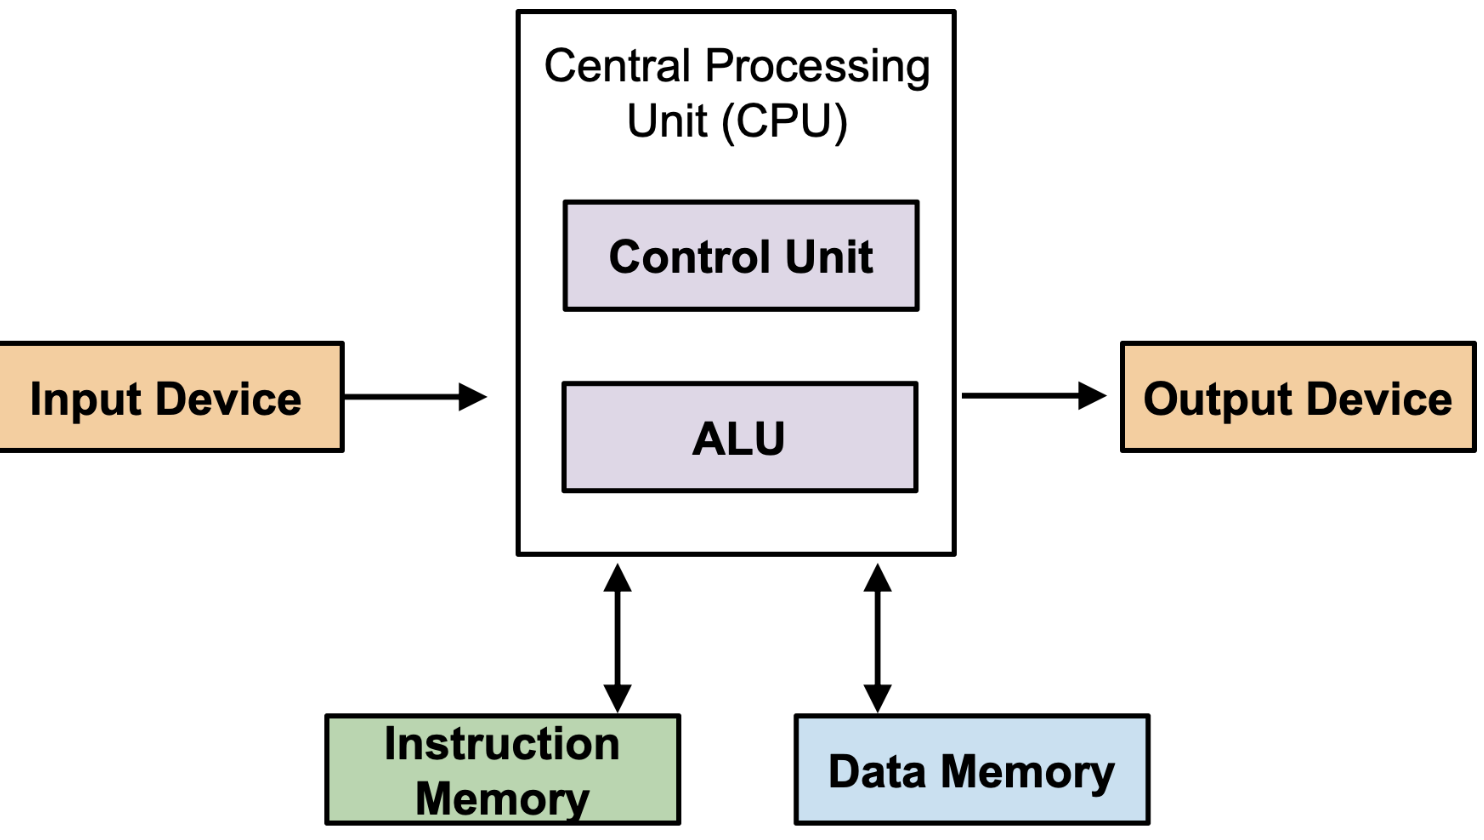
\includegraphics[scale=0.2]{harvard-architecture}
\subsubsection{Von Neumann architecture}
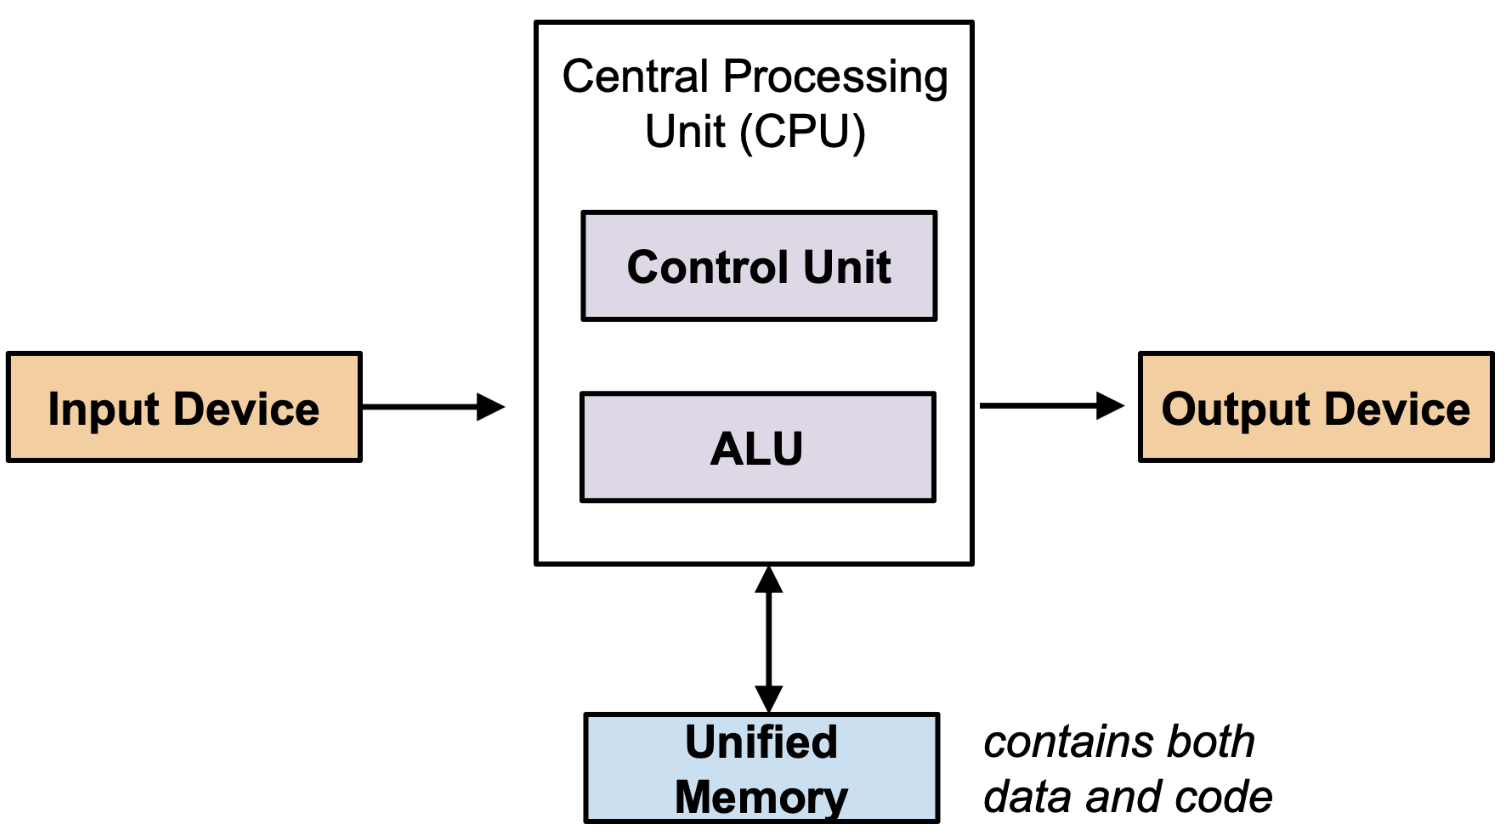
\includegraphics[scale=0.2]{von-neumann}

\begin{description}
	\item[Difference]{Separate vs common storage pathway for code and data}
\end{description}
Why do we need OS?

\subsection{Mainframe}
Old analog "computers" using physical cards for programming
\subsubsection{Improvements}
\begin{itemize}
	\item Problem: Batch processing inefficient
	\item Solution: Multiprogramming
	\begin{itemize}
		\item Loading multiple jobs that runs while other jobs using I/O
		\item Overlapping computation with I/O
	\end{itemize}
	\item Problem: Only one user 
	\item Solution: Time sharing OS
	\begin{itemize}
		\item Multiple concurrent users using terminals
		\item User job scheduling 
		\item Memory management
		\item \keyword{Hardware virtualization}{Each program executes as if it had all resources}
	\end{itemize}
\end{itemize}


\subsection{Motivation}
\begin{enumerate}
	\item Abstraction
	\begin{itemize}
		\item Hide low level details and present common, high-level functionality to users
	\end{itemize}
	\item Resource allocation
	\begin{itemize}
		\item Allow concurrent usage of resource and execute programs simultaneously
		\item Arbitrate conflicting request fairly and efficiently
	\end{itemize}
	\item Control programs
	\begin{itemize}
		\item Restrict resource allocation
		\item Security, protection and error prevention
		\item Ensure proper use of device
	\end{itemize}
\end{enumerate}
\subsubsection{Advantage}
\begin{itemize}
	\item Portable and flexible
	\item Use computer resources efficiently
\end{itemize}
\subsubsection{Disadvantage}
\begin{itemize}
	\item Significant overhead
\end{itemize}

\subsubsection{OS vs User Program}
Similarities
\begin{itemize}
	\item Both softwares
\end{itemize}
Difference
\begin{itemize}
	\item OS runs in \keyword{kernel mode}{Access to all hardware resources}
	\item User programs run in \keyword{User mode}{Limited access}
	\item User programs use syscalls to communicate with OS for hardware processes
\end{itemize}
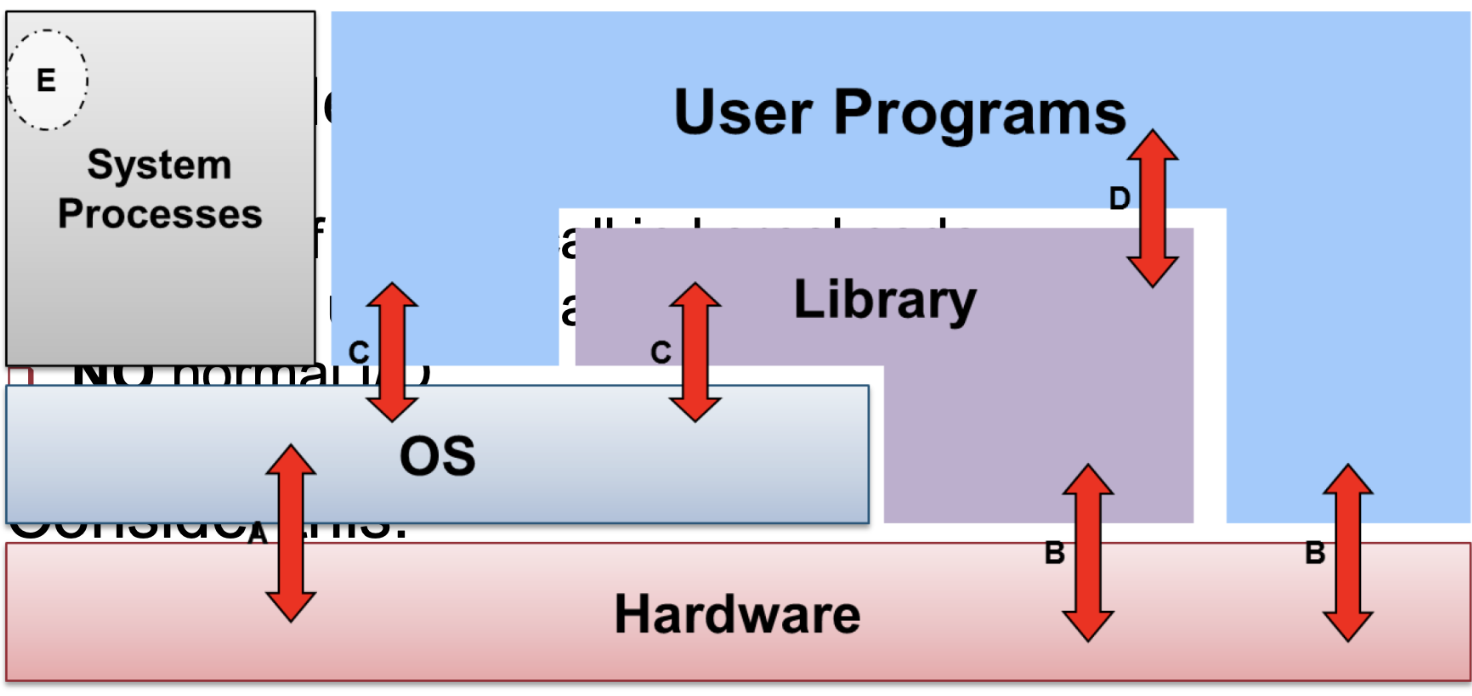
\includegraphics[scale=0.2]{os-interaction}
\\Why OS dont occupy entire hardware layer
\begin{itemize}
	\item Slow to have all operations pass through intermediary
	\item User programs can have direct interaction with hardware (eg. Arithmetic) during low risk operations
\end{itemize}

\subsection{OS structure}
\subsubsection{Monolithic OS}
\begin{itemize}
	\item One big kernel program
	\item Well understood and has good performance
	\item Highly \keyword{coupled}{internal structure interconnected that unintentionally affect each other}
\end{itemize}
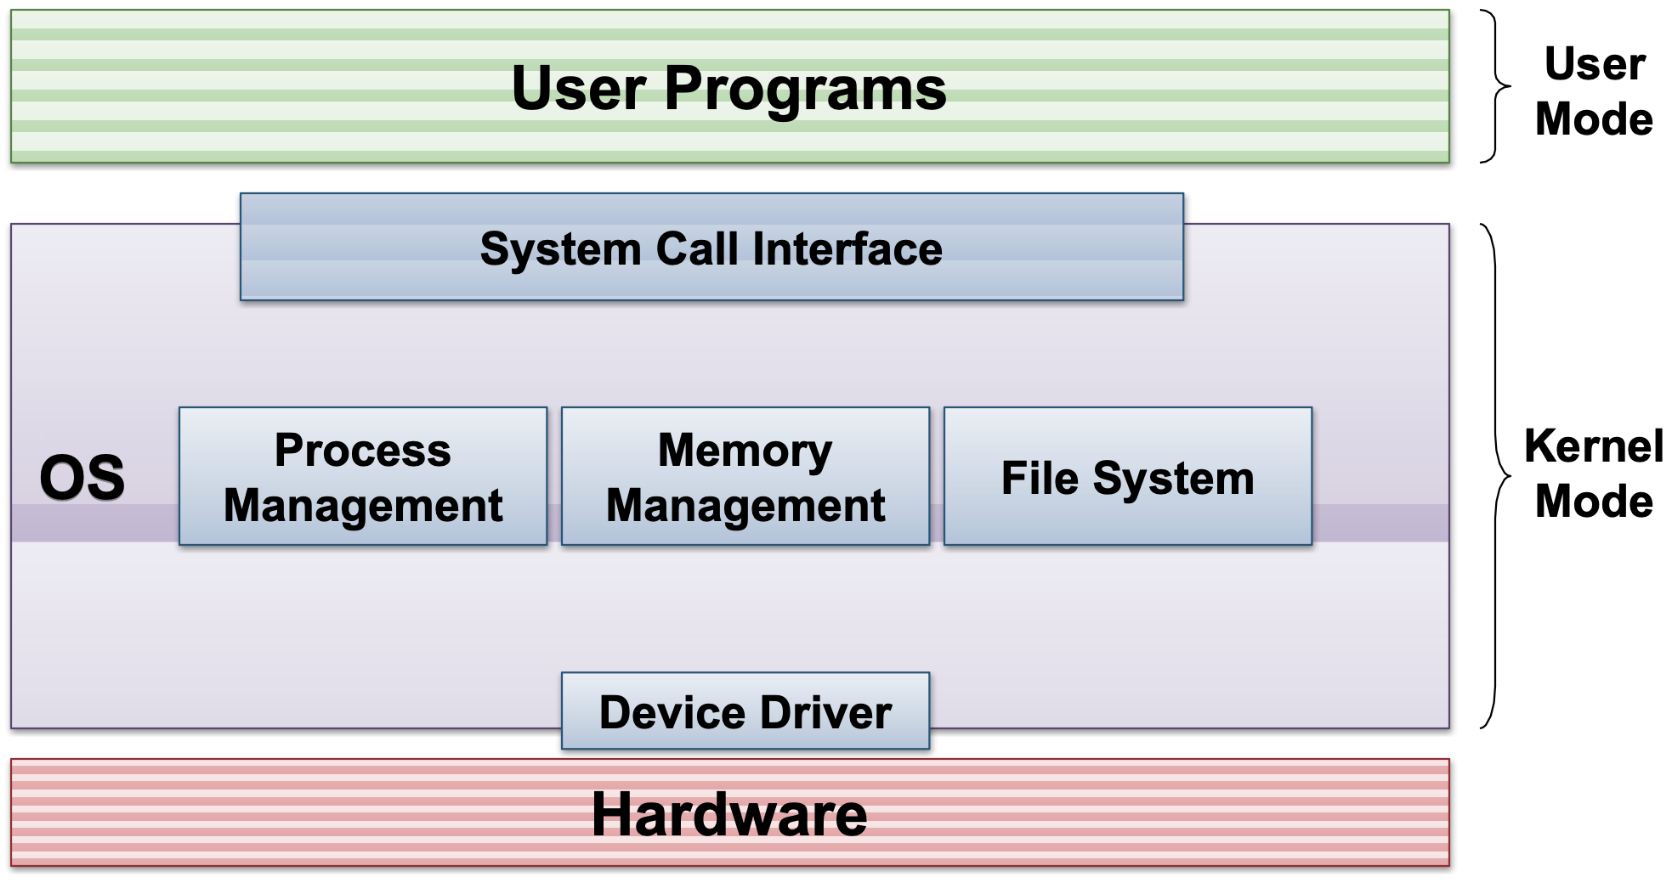
\includegraphics[scale=0.2]{monolithic-os}

\subsubsection{Microkernel}
\begin{itemize}
	\item Small clean
	\item Basic and essential facilities
	\item IPC communication OR run external programs outside OS
	\item Robust and more \keyword{modular}{Extendible and maintainable}
	\item Better isolation btw kernel and services
	\item Lower performance
\end{itemize}
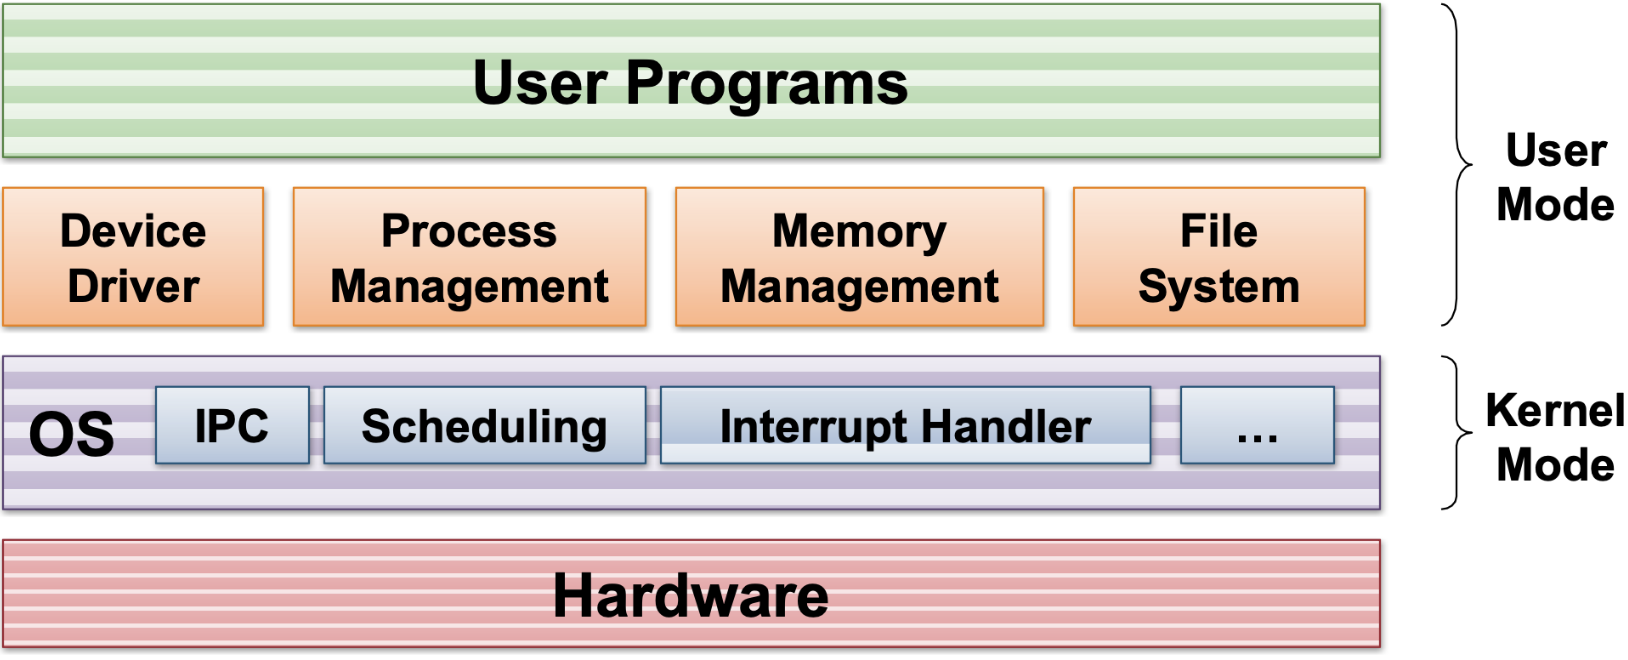
\includegraphics[scale=0.2]{microkernel-os}
%--------------------------------------------------------------------------------------------------------------------
%--------------------------------------------------------------------------------------------------------------------
%--------------------------------------------------------------------------------------------------------------------
%--------------------------------------------------------------------------------------------------------------------
%--------------------------------------------------------------------------------------------------------------------
\end{multicols*}
\end{document}